
%(BEGIN_QUESTION)
% Copyright 2011, Tony R. Kuphaldt, released under the Creative Commons Attribution License (v 1.0)
% This means you may do almost anything with this work of mine, so long as you give me proper credit

One extremely useful capability of a ``smart'' valve positioner is the ability to measure and plot the relationship between valve stem position and actuator air pressure.  Sketch what a ``healthy'' {\it valve signature} should look like, assuming a valve with the following properties:

$$\includegraphics[width=15.5cm]{i01539x01.eps}$$

\begin{itemize}
\item{} Stem-guided globe trim
\vskip 10pt
\item{} Reverse-acting pneumatic actuator
\vskip 10pt
\item{} Direct-acting valve body
\vskip 10pt
\item{} Equal-percentage trim characteristic
\vskip 10pt
\item{} 6 PSI lower bench-set pressure
\vskip 10pt
\item{} 15 PSI upper bench-set (end-of-stroke) pressure
\end{itemize}

\vskip 20pt \vbox{\hrule \hbox{\strut \vrule{} {\bf Suggestions for Socratic discussion} \vrule} \hrule}

\begin{itemize}
\item{} Identify some of the control valve problems that may be diagnosed by skillful examination of a valve signature plot.
\end{itemize}

\underbar{file i01539}
%(END_QUESTION)




%(BEGIN_ANSWER)


%(END_ANSWER)





%(BEGIN_NOTES)

This valve signature is {\it ideal}, showing no friction at all:

$$\includegraphics[width=15.5cm]{i01539x02.eps}$$

The fact that the trim is equal-percentage is irrelevant information, but it might cause some students to try and sketch the valve signature as a {\it curve}.  The fact that this valve is stem-guided does not affect the signature either.

Technically, the fact that the valve body is direct-acting is relevant because it tells where the {\it seating profile} will be found on this valve.  However, the crude valve signature I show doesn't give that level of detail and so we can say the valve body's action is irrelevant for the scope of this question.



\vskip 20pt \vbox{\hrule \hbox{\strut \vrule{} {\bf Suggestions for Socratic discussion} \vrule} \hrule}

\begin{itemize}
\item{} Explain why it would be incorrect to sketch this function as a curve, in an effort to reflect equal-percentage valve characterization.
\end{itemize}

%INDEX% Final Control Elements, valve: diagnostic signature for pneumatic actuator

%(END_NOTES)


